\documentclass{article}
\usepackage{multicol}
\usepackage{graphicx}% Include figure files
\usepackage{dcolumn}% Align table columns on decimal point
\usepackage{bm}% bold math
\usepackage{hyperref}% add hypertext capabilities
\usepackage{booktabs}
\usepackage{listings}
\usepackage{mathtools}
\usepackage{amsmath}
\usepackage{amssymb}
\usepackage{multirow}
\renewcommand{\abstractname}{\vspace{-\baselineskip}}
\bibliographystyle{plain}
\usepackage[utf8]{inputenc}
\usepackage{verbatim} %for å inkludere filer med tegn LaTeX ikke liker
\DeclareMathAlphabet      {\mathbfit}{OML}{cmm}{b}{it}
\usepackage{mathpazo}
\usepackage{float}
\usepackage{algpseudocode}
\newcommand\numberthis{\addtocounter{equation}{1}\tag{\theequation}}
\usepackage[left=20mm,right=20mm,top=33.95mm,bottom=33.95mm]{geometry} 
% Justerer bredden på columns.
\setlength{\columnsep}{1cm}

\usepackage{amsmath,systeme}

\sysalign{r,r}

\begin{document}

\title{{Background Cosmology}}
\author{{Andreas Wetzel}}

\maketitle
\begin{multicols}{2}
\section{Introduction}
In this project we are going to look at the uniform background in the Universe and investigate the expansion history of the universe. We will do this by computing the expansion history of the universe numerical and analytical, and observe the uniform background densities for different components of matter and energy.  
\section{Theoretical background}
A uniform background universe describes the spatial distribution of matter to be homogeneous and isotropic observed at a large scale. This is also known as the Cosmological Principle. In this project we assume that the universe is flat which means that $k=0$ in the Friedmann–Lemaître–Robertson–Walker metric (FRLW)
\begin{align}
    ds^2 =-dt^2+a(t)^2(dx^2+dy^2+dz^2)\label{FLRW_cart}
\end{align}
Where equation \eqref{FLRW_cart} is in Cartesian coordinates. $a(t)$ is the only free variable in equation \eqref{FLRW_cart}, and it tells us how fast the Universe expands and how object behaves. To be able to evaluate the expansion of the Universe, we have to insert the metric \eqref{FLRW_cart} into the Friedmann equation, which is given in equation \eqref{eq:Friedmann_eq}
\begin{align}
    H=H_0\sqrt{(\Omega_{b0}+\Omega_{\text{CDM}0})a^{-3}+(\Omega_{\gamma0}+\Omega_{\nu0})a^{-4}\Omega_{k0}a^{-2}+\Omega_{\Lambda0}} \label{eq:Friedmann_eq}
\end{align}
for simplicity we say that $\Omega_{m0}=(\Omega_{b0}+\Omega_{\text{CDM}0})$ and $\Omega_{r0}=(\Omega_{\gamma0}+\Omega_{\nu0})$, further we
have the Hubble parameter, $H=\frac{da}{dt}\frac{1}{a}=\frac{\Dot{a}}{a}$ and the $\Omega$-values, which describes the relative densities for present day. $\Omega_{b0}\approx 0.05$ is for baryonic matter, $\Omega_{\text{CDM}0}\approx 0.25$ is for dark matter, $\Omega_{\gamma0}$ is for radiation, $\Omega_{\nu0}$ is for the neutrino energy and $\Omega_{\Lambda 0}\approx 0.7$ is for dark energy. The $\Omega_{k0}=-\frac{kc^2}{H_0^2}$ term describes the curvature, by setting $a=1$ we have that $\Omega_{k0}=1-\Omega_{m0}-\Omega_{r0}-\Omega_{\Lambda0}$. Since we don't include curvature we set $\Omega_{k0}=0$. 
Further we have that the radiation parameter and the neutrino energy is given as 
\begin{align}
    \Omega_{\gamma0}&= 2\cdot \frac{\pi^2}{30}\frac{(k_bT_{\text{CDM}0})^4}{\hbar^3c^5}\frac{8\pi G}{3H_0^2}\\
    \Omega_{\nu0}&=N_\text{eff}\cdot\frac{7}{8}\bigg(\frac{4}{11}\bigg)^\frac{4}{3}\Omega_{\gamma0}
\end{align}
where $T_{\text{CDM}0}=2.7255$K is today's temperature of the CMB, and $N_\text{eff}=3.0466$ is the effective number of neutrinos. \\
All these components and equation \eqref{eq:Friedmann_eq} is known as the standard model of cosmology.\\   
\\
We can also write the Friedmann equation on the following form
\begin{align}
    H=H_0=\sqrt{\frac{\rho_x}{\rho_c}} \label{eq:H_rho}
\end{align}
where $\frac{\rho_x}{\rho_c}=\Omega_{m0}+\Omega_{r0}+\Omega_{k0}+\Omega_{\Lambda 0}$ and $\rho_c=3H^2/(8\pi G)$.\\
The Friedmann equation can show us how each density components changes with time, this is given by the following equation
\begin{align}
    \Dot{\rho}+3H(\rho+P)=0
\end{align}
where $\rho$ is the density and $P$ is the pressure. This equation tells us how the components evolves over time. There is also the equation of state which is given as

    $\omega=\frac{P}{\rho}$ and $\omega$ will be constant.
Hence we have that 
\begin{align}
    \rho\propto a^{-3(1+\omega)}
\end{align}
Where
\begin{equation}
\omega=
\systeme{
  0\;\;\;\; \text{for cold dark matter and baryons},
  1/3\;\;\;\; \text{for radiation} \;\;\;\;\;\;\;\;\;\;\;\;\;\;\;\;\;\;\;\;\;\;\;\;\;\;\;\;\;,
  -1\;\;\;\; \text{for dark energy}\;\;\;\;\;\;\;\;\;\;\;\;\;\;\;\;\;\;\;\;\;\;\;\;\;
} \label{eq:omega_val}
\end{equation}
\\
\\
When we look at the cosmic microwave background, CMB, it is important to look at the \emph{comoving horizon}. Comoving horizon tells us how far the light has travelled after the Big Bang, where $t=0$. The comoving horizons expands with time, which we call \emph{conformal time}, $\eta$. We can write the conformal time in the following form
\begin{align}
    \frac{d\eta}{dt}&=\frac{c}{a}\label{eq:deta_t}\\
    &=\frac{d\eta}{da}\frac{da}{dt}\\
    &=\frac{d\eta}{da}aH \label{eq:deta_a}
\end{align}
We are now able to write $\eta$ as a function $x$ by using equation \eqref{eq:deta_t} and \eqref{eq:deta_a}
\begin{align}
    \frac{d\eta}{da}&=\frac{c}{a^2H}=\frac{c}{a\mathcal{H}}\\
    \frac{d\eta}{dx}&=\frac{da}{dx}\frac{d\eta}{da}=\frac{c}{\mathcal{H}}\\
    \eta(x)&=\int_{-\infty}^x\frac{cdx'}{\mathcal{H}(x')} \label{eq:eta_x}
\end{align}
where $\mathcal{H}=aH$ is a scaled version of the Hubble parameter.
\begin{align}
    \mathcal{H}=aH_0\sqrt{\Omega_{m0}a^{-3}+\Omega_{r0}a^{-4}\Omega_{k0}a^{-2}+\Omega_{\Lambda0}} \label{eq:Friedmann_eq_Hp}
\end{align}
There are several ways to measure the time in our Universe. One of these is the relation between time and scale factor. They have a one-to-one relation, which means we can use the scale factor to calculate the time.\\
 Another way to calculate time is to use the redshift, which is done by measuring the time by observing how far the wavelength of a photon has been extended after it was sent out at a time $t$.
\\
There are other ways to calculate the distances in the Universe as well. The calculations on the distances depends on the geometry.
 We are only going to look at the measurement on a flat universe, and one of the methods to calculate the distance is called \emph{comoving distance}. It excludes the expansion of then universe. Due to the expansion of space will a given distance not change over time. And with a given redshift $z$ can we write the comoving distance as
\begin{align}
    \chi &=\int_1^a\frac{cda}{a^2H}=\int_0^z\frac{cdz}{H}\\
    &=\eta-\eta_0
\end{align}
where
\begin{align}
    \chi=\int_t^{t_\text{today}}\frac{cdt}{a}=r
\end{align}
and $\frac{cdt}{a}=dr$ if a photon moves radially to us in a flat universe.
\\
There is also distance measure that is called \emph{angular distance measure}. This is a distance that is defined at the size, $\Delta s$, of an object with a given redshift which has an angular size $\Delta \theta$. It can be written in the following form
\begin{align}
    d_A=\frac{\Delta s}{\Delta \theta}=\frac{S_k(r)}{1+z}
\end{align}
where $S_k(r)=\chi$.\\
Another distance measure is the luminosity distance, this distance can be calculated by finding the flux, $F$, and the luminosity, $L$, and is given as
\begin{align}
    d_L=\sqrt{\frac{L}{4\pi F}}
\end{align}
we know the that $L\propto \frac{1}{a^4}$ and $F\propto\frac{1}{d_A^2}$, and we can therefore see a relation between luminosity distance and angular distance 
\begin{align}
    d_L&=\sqrt{\frac{1/a^4}{1/d_A^2}}\\
    &=\frac{d_A}{a^2}
\end{align}

\section{Method}
By calculating expansion history of the universe numerical we us a model which contains the cosmological parameters and functions which will give use the conformal time, distance measure and the Hubble parameter. As our time variable we will use the scale factor $a=e^{x}$.   
\\
We will compute and make plots of $H(x)$, $\mathcal{H}(x)$, $\frac{1}{\mathcal{H}(x)}\frac{d\mathcal{H}(x)}{dx}$, $\frac{1}{\mathcal{H}(x)}\frac{d^2\mathcal{H}(x)}{dx^2}$, $\eta(x)$, $\frac{\eta(x) is \mathcal{H}(x)}{c}$, $t(x)$, $\Omega_m$, $\Omega_r$ and $\Omega_\Lambda$, we use different functions for all the $\Omega$-values, which you can see below. 
\begin{align}
    \Omega_{k}(a)&=\frac{\Omega_{k0}}{a^2H(a)^2/H_0^2} \label{eq:Omega_k}\\
    \Omega_{\text{CDM}}(a)&=\frac{\Omega_{\text{CDM}0}}{a^2H(a)^2/H_0^2} \label{eq:Omega_CDM}\\
    \Omega_{b}(a)&=\frac{\Omega_{n0}}{a^3H(a)^2/H_0^2} \label{eq:Omega_b}\\
    \Omega_{\gamma}(a)&=\frac{\Omega_{\gamma0}}{a^4H(a)^2/H_0^2} \label{eq:Omega_gamma}\\
    \Omega_{\nu}(a)&=\frac{\Omega_{\nu0}}{a^4H(a)^2/H_0^2} \label{eq:Omega_nu}\\
    \Omega_{\Lambda}(a)&=\frac{\Omega_{\Lambda0}}{a^4H(a)^2/H_0^2} \label{eq:Omega_lambda}
\end{align}
\subsection{Position, redshift and time }
First of all we want calculate the times - $x$, $z$, $t$ for radiation-matter equality, matter-dark energy equality and when the Universe starts to accelerate. We will use these values to mark the transitions between the different phases and see how this effects the universe in different settings.\\
We start to compute the time for radiation-matter equality, $\Omega_{m}=\Omega_{r}$. We now that $\Omega_{m0}\propto a^{-3}$ and $\Omega_{r0}\propto a^{-4}$ we then get the equation
\begin{align}
    a^{-3}\Omega_{m0}&=a^{-4}\Omega_{r0}\\
    a_{MR}&=\frac{\Omega_{r0}}{\Omega_{m0}} \label{eq:a_MR}
\end{align}
Further we compute the time for matter-dark energy equality, $\Omega_{m}=\Omega_{\Lambda}$, and we have that $\Omega_{\Lambda}\propto 1$, which gives us
\begin{align}
    a^{-3}\Omega_{m0}&=\Omega_{\Lambda0}\\
    a_{MDE}&=\bigg(\frac{\Omega_{m0}}{\Omega_{\Lambda0}}\bigg)^{\frac{1}{3}} \label{eq:a_mde}
\end{align}
Finally we compute when the Universe starts to accelerate. We have that 
\begin{align}
    \Dot{a}=aH&=\sqrt{\Omega_{m0}a^{-3}+\Omega_{\Lambda0}}\\
    &=H_0\sqrt{\Omega_{m0}a^{-1}+\Omega_{\Lambda0} a^2}
\end{align}
This gives us now 
\begin{align}
    \Ddot{a}&=H_0\frac{1}{2}\frac{1}{\sqrt{\Omega_{m0}a^{-1}+\Omega_{\Lambda0} a^2}}\bigg(\Omega_{m0}\bigg(-\frac{1}{a^2}\bigg)\Dot{a}+2\Omega_{\Lambda0} a\Dot{a}\bigg)=0
\end{align}
We simplify this expression by cancelling out some values. This gives us
\begin{align}
    \Ddot{a}=\bigg(-\Omega_{m0}\frac{\Dot{a}}{a^2}+2\Omega_{\Lambda0} a\Dot{a}\bigg)&=0\\
    -\Omega_{m0}\frac{1}{a^2}+2\Omega_\Lambda a&=0\\
    2\Omega_{\Lambda0} a&=\Omega_{m0}\frac{1}{a^2}\\
    a&=\bigg(\frac{\Omega_{m0}}{\Omega_{\Lambda0}}\bigg)^\frac{1}{3} \label{eq:a_acc}
\end{align}
\\
We now insert equation \eqref{eq:a_MR}, \eqref{eq:a_mde} and \eqref{eq:a_acc} into equation \eqref{eq:x}-\eqref{eq:t} which will then gives us the different values for position, redshift and time for radiation-matter equality, matter-dark energy equality and when the Universe starts to accelerate.
\begin{align}
    x=\ln{a} \label{eq:x}\\
    z = \frac{1}{a}-1 \label{eq:z}\\
    t=t(\ln{a}) \label{eq:t}
\end{align}
\subsection{$H$ and $\mathcal{H}$}
We will now compute $H$, so we use equation \eqref{eq:Friedmann_eq} which is written as 
\begin{align}
     H(x)=H_0\sqrt{\Omega_{m0}e^{-3x}+\Omega_{r0}e^{-4x}\Omega_{k0}e^{-2x}+\Omega_{\Lambda0}} \label{eq:H_x}
\end{align}
as a function of x.\\
We insert equation \eqref{eq:Omega_k}-\eqref{eq:Omega_lambda} into equation \eqref{eq:H_x}.\\
To compute $\mathcal{H}$ we use equation \eqref{eq:Hp_eq}  
\begin{align}
    \mathcal{H}(x)&=e^xH_0\sqrt{{\Omega_{m0}e^{-3x}+\Omega_{r0}e^{-4x}\Omega_{k0}e^{-2x}+\Omega_{\Lambda0}}}\\
    &=H_0\sqrt{\Omega_{m0}e^{-x}+\Omega_{r0}e^{-2x}+\Omega_{k0}+\Omega_{\Lambda0}e^{2x}}\label{eq:Hp_eq}
\end{align}
and we will say that $$\Omega_{v1}=\Omega_{m0}e^{-x}+\Omega_{r0}e^{-2x}+\Omega_{k0}+\Omega_{\Lambda0}e^{2x}$$ which gives us \begin{align}
     \mathcal{H}(x)=H_0\sqrt{\Omega_{v1}} \label{eq:Hp_x_omega}
\end{align}  
\subsection{$\frac{1}{\mathcal{H}(x)}\frac{d\mathcal{H}(x)}{dx}$ and $\frac{1}{\mathcal{H}(x)}\frac{d^2\mathcal{H}(x)}{dx^2}$}
I chose to solve $\frac{1}{\mathcal{H}(x)}\frac{d\mathcal{H}(x)}{dx}$ and $\frac{1}{\mathcal{H}(x)}\frac{d^2\mathcal{H}(x)}{dx^2}$ analytically, and we therefore start to use derivation on equation \eqref{eq:Hp_x_omega}
\begin{align}
    \frac{d\mathcal{H}(x)}{dx}&=H_0\frac{1}{2}\frac{1}{\sqrt{\Omega_{v1}}}\Omega_{v1}'\\
    &=H_0\frac{1}{\sqrt{\Omega_{v1}}}(-\Omega_{m0}e^{-x}-2\Omega_{r0}e^{-2x}+\Omega_{k0}+2\Omega_{\Lambda0}e^{2x})\\
    &=H_0\frac{1}{2}\frac{1}{\sqrt{\Omega_{v1}}}\Omega_{v2} \label{eq:dHp_dx}
\end{align}
where $$\Omega_{v2}=(-\Omega_{m0}e^{-x}-2\Omega_{r0}e^{-2x}+\Omega_{k0}+2\Omega_{\Lambda0}e^{2x})$$\\
We are now able to calculate $\frac{1}{\mathcal{H}(x)}\frac{d^2\mathcal{H}(x)}{dx^2}$ by finding the derivative of equation \eqref{eq:dHp_dx}.
\begin{align}
   \frac{d^2\mathcal{H}(x)}{dx^2}&=\frac{1}{2}H_0(\Omega_{v2}'\Omega_{v1}^{-1/2}+\Omega_{v2}(\Omega_{v2}^{-1/2})' )\\
   &=\frac{1}{2}H_0\bigg(\frac{\Omega_{m0}e^{-x}+4\Omega_{r0}e^{-2x}+\Omega_{k0}+4\Omega_{\Lambda0}e^{2x}}{\Omega_{v1}}\nonumber\\&+\Omega_{v2}\bigg(-\frac{1}{2}\frac{1}{\Omega_{v1}^{3/2}}\Omega_{v1}'\bigg)\bigg)
\end{align}
we now say that $$\Omega_{v3}=\Omega_{m0}e^{-x}+4\Omega_{r0}e^{-2x}+\Omega_{k0}+4\Omega_{\Lambda0}e^{2x}$$ 
This will then give us
\begin{align}
    \frac{d^2\mathcal{H}(x)}{dx^2}&=\frac{1}{2}H_0\bigg(\frac{\Omega_{v3}}{\sqrt{\Omega_{v1}}}-\frac{1}{2}\frac{\Omega_{v2}}{{\Omega_{v1}^{3/2}}}\Omega_{v2}\bigg)\\
    &=\frac{1}{2}H_0\frac{1}{\sqrt{\Omega_{v1}}}\bigg(\Omega_{v3}-\frac{1}{2}\frac{\Omega_{v2}^2}{\Omega_{v1}}\bigg)
\end{align}
We have now found values for $\frac{d\mathcal{H}(x)}{dx}$ and $\frac{d^2\mathcal{H}(x)}{dx^2}$ analytically and we now insert these values into two function and dived each of them with $\mathcal{H}(x)$.\\
\subsection{$\eta(x)$ and $t(x)$}
To compute $\eta(x)$ and $t(x)$ we use the 4th-Order Runge Kutta for solving our ODEs. After we solved the ODEs we made a cubic spline which gives us the values for $\eta(x)$ and $t(x)$.\\
Now that we have computed $\eta(x)$ and $t(x)$ we will find the age of the Universe today, $t(0)$, and the conformal time today, $\eta(0)/c$.
\subsection{$\Omega$-values}
For the calculation and plotting for $\Omega_{m}=\Omega_{b}(x)+\Omega_{\text{CDM}}(x)$ we just sum the equations \eqref{eq:Omega_b} and \eqref{eq:Omega_CDM}, the same goes $\Omega_{r}=\Omega_{\gamma}(x)+\Omega_{\nu}(x)$, we just sum equation \eqref{eq:Omega_gamma} and \eqref{eq:Omega_nu}. For $\Omega_{\Lambda}(x)$ we just use the equation \eqref{eq:Omega_lambda}. 
\section{Results}
We computed $x$, $z$ and $t$ for the radiation-matter equality, (RM), matter-dark energy equality, (MDE), and when the universe starts to accelerate, (AccU). We can see these values in the table below.
\begin{center}
\begin{tabular}{ |c||c|c|c| } 
 \hline
 &RM & MDE & AccU \\ 
 \hline
 \hline
 x & -8.669 & -0.256&-0.487 \\ 
 \hline
 z & 5822 & 0.291&0.627 \\ 
 \hline
  t [\text{Gyr}] & 2.266$\cdot10^{-5}$ & 10.319& 7.708 \\ 
 \hline
\end{tabular}
\end{center}
Table 1: Overview of the values $x$, $z$ and $t$ when we have radiation-matter equality, matter-dark energy equality and at the point where the universe starts to accelerate. 
\begin{figure}[H]
	\centering
	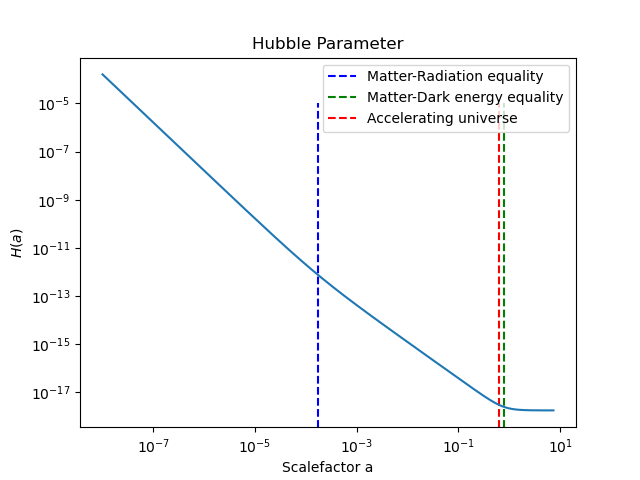
\includegraphics[width=77mm]{Hubble Parameter.png}
	\caption{The evolution of the Hubble parameter.}
	\label{fig:H(x)}
\end{figure}
We see in figure \eqref{fig:H(x)} that the Hubble parameter decreases most of the time. If we start by looking at the period where radiation where the dominant density we can see that the Hubble parameter decreases the most, this makes sense as we look at equation \eqref{eq:Friedmann_eq}, and see that $H\propto \frac{1}{a^2}$. As time passes and we move into the period where matter was the dominant density we see that the Hubble parameter still decreases, but not as sharp as in the radiation period, the reason for this is that $H\propto \frac{1}{\sqrt{a^3}}$.
When we go towards our present time we see an era where the dominant density in out Universe is dark energy. We know that $H\propto 1$ in the dark energy dominant era, hence we see that the Hubble parameter stays constant as in figure \eqref{fig:H(x)}. In the plot we can also see that the universe starts to accelerate  right before we meet the Matter-Dark energy equality. 
\begin{figure}[H]
	\centering
	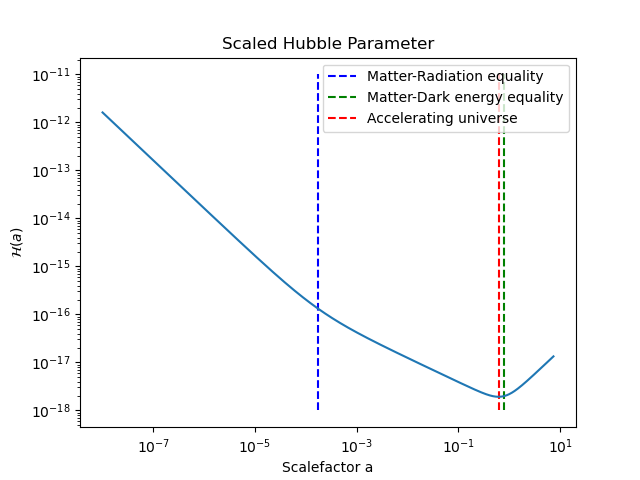
\includegraphics[width=77mm]{Scaled Hubble Parameter.png}
	\caption{The evolution of the scaled Hubble parameter}
	\label{fig:Hp(x)}
\end{figure}
Also in figure \eqref{fig:Hp(x)} we see that scaled Hubble parameter decreases, but this one decreases slower than $H$. This comes from that $\mathcal{H}\propto \frac{1}{a}$ for radiation dominated time, for matter dominated time $\mathcal{H}$ decreases slower than the  radiation dominated time, this comes from that $\mathcal{H}\propto \frac{1}{\sqrt{a}}$. For the dark energy dominated time will $\mathcal{H}$ start to increase, due to $\mathcal{H}\propto {a}$ for dark energy dominated time. \\
\\
In figure \eqref{fig:der_Hp(x)} we see the behaviour of the first and second derivative of $\mathcal{H}$, the most interesting thing about this figure is to see what happens at $\frac{d\mathcal{H}}{dx}=0$. At this point we see that the universe starts to accelerate. By using equation \eqref{eq:H_rho} we found $\frac{d\mathcal{H}}{dx}/H$ and $\frac{d^2\mathcal{H}}{dx^2}/H$
\begin{figure}[H]
	\centering
	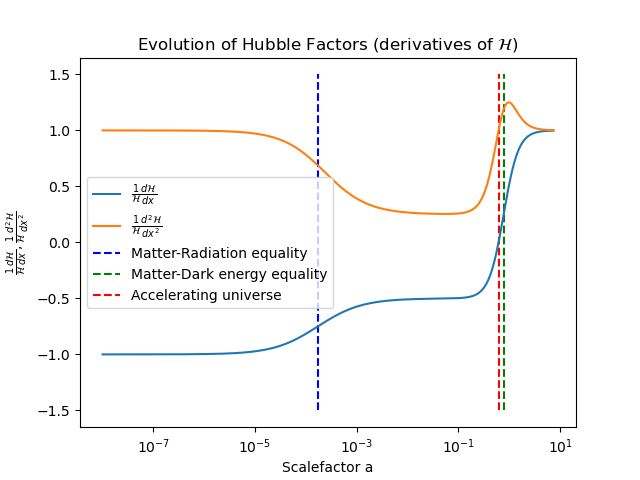
\includegraphics[width=77mm]{der_Hp.png}
	\caption{The behavior of the first and second derivatives of $\mathcal{H}$ as the scalefactor increases.}
	\label{fig:der_Hp(x)}
\end{figure}
\begin{align}
    \frac{d\mathcal{H}(x)}{dx}/H&=-\frac{1}{2}(1+3\omega) \label{eq:der_H_om}\\
    \frac{d^2\mathcal{H}(x)}{dx^2}/H&=\frac{1}{4}(1+3\omega)^2 \label{eq:der_H2_om}
\end{align}
See appendix \eqref{A.1} for the calculation.\\
If we now insert equation \eqref{eq:omega_val} into \eqref{eq:der_H_om} and \eqref{eq:der_H2_om} we get
\begin{equation}
\frac{d\mathcal{H}(x)}{dx}/H=
\systeme{
  -\frac{1}{2}\;\;\;\; \text{for cold dark matter and baryons},
  -1\;\;\;\; \text{for radiation} \;\;\;\;\;\;\;\;\;\;\;\;\;\;\;\;\;\;\;\;\;\;\;\;\;\;\;\;\;\;\;\;\;,
  1\;\;\;\; \text{for dark energy}\;\;\;\;\;\;\;\;\;\;\;\;\;\;\;\;\;\;\;\;\;\;\;\;\;\;\;\;\;
} \label{eq:derH_inserted}
\end{equation}
\begin{equation}
\frac{d^2\mathcal{H}(x)}{dx^2}/H=
\systeme{
  \frac{1}{4}\;\;\;\; \text{for cold dark matter and baryons},
  1\;\;\;\; \text{for radiation} \;\;\;\;\;\;\;\;\;\;\;\;\;\;\;\;\;\;\;\;\;\;\;\;\;\;\;\;\;\;\;\;\;,
  1\;\;\;\; \text{for dark energy}\;\;\;\;\;\;\;\;\;\;\;\;\;\;\;\;\;\;\;\;\;\;\;\;\;\;\;\;
} \label{eq:derH2_inserted}
\end{equation}
So if we look at equation \eqref{eq:derH_inserted} we see that $\frac{d\mathcal{H}(x)}{dx}/H$ should be at $-1$ for the radiation dominated time, and as it moves to the matter-dominated time it should be $-\frac{1}{2}$ and $1$ at the dark energy-dominated time. So these values indicates that the $\frac{d\mathcal{H}(x)}{dx}/H$ plot looks right. For the $\frac{d^2\mathcal{H}(x)}{dx^2}/H$ we found that it should be $1$ for radion-dominated time, $\frac{1}{4}$ for matter-dominated time and $1$ for dark energy-dominated time as we can see in equation \eqref{eq:derH2_inserted}. These values also fits our plot for $\frac{d^2\mathcal{H}(x)}{dx^2}/H$.  
\begin{figure}[H]
	\centering
	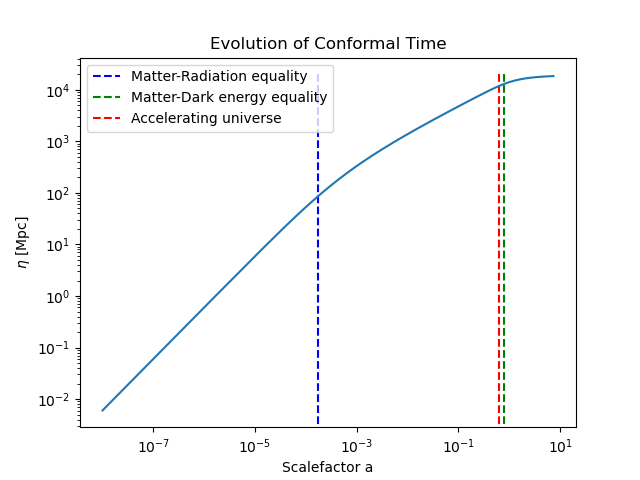
\includegraphics[width=77mm]{Evolution of Conformal Time.png}
	\caption{The conformal time $\eta$. Shows the evolution of the universe}
	\label{fig:Ev_Conf_time(x)}
\end{figure}
\begin{figure}[H]
	\centering
	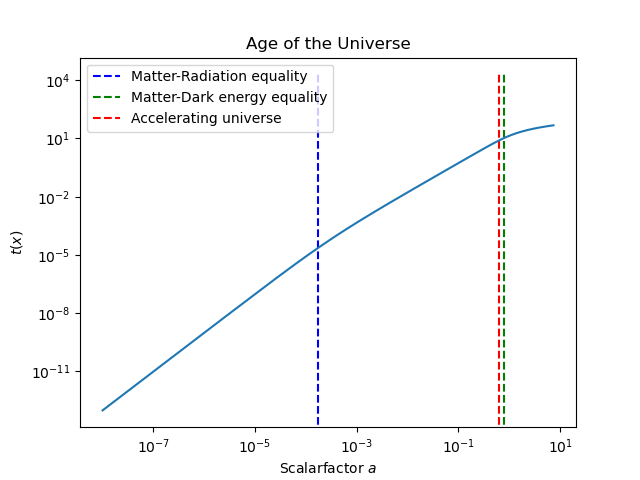
\includegraphics[width=77mm]{t_of_x.png}
	\caption{The age of the universe as a function of the scalefactor}
	\label{fig:t_of_x}
\end{figure}
We now that $\eta \propto a$ in the radiation dominated time. This indicates that figure \eqref{fig:Ev_Conf_time(x)} looks right since $\eta$ is moving linear with the scalar factor in the radiation dominated time. For the matter dominated time we have that $\eta\propto \sqrt{a}$. And our figure here also looks right since $\eta$ still increases as we move in the matter dominated time, but not as sharply when radiation was the dominant density. In the dark energy dominated time will $\eta \propto 1$, hence will $\eta$ move constant horizontal as in figure \eqref{fig:Ev_Conf_time(x)}. And we find that the Conformal time today is 
\begin{align}
    \eta(0)=46.25\text{Gyr}
\end{align}
We see in figure \eqref{fig:t_of_x} that when we reach the time where  dark energy is the dominated density, that the universe does not expand constant anymore. The expansion is now accelerating! We also find the age of the universe today, which is
\begin{align}
    t(0)=13.77 \text{Gyr}
\end{align}
which is a reasonable number.
\begin{figure}[H]
	\centering
	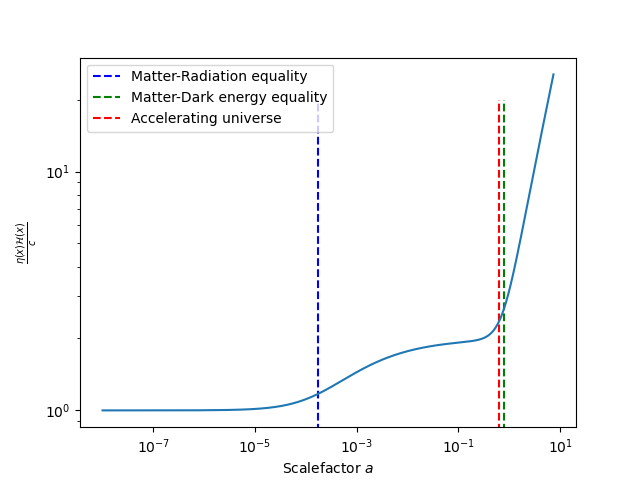
\includegraphics[width=77mm]{eta_Hp_c.png}
	\caption{Checking the values of $\eta$ and $\mathcal{H}$}
	\label{eq:eta_Hp_c}
\end{figure}
Figure \eqref{eq:eta_Hp_c} is just a test to see if the values for $\eta$ and $\mathcal{H}$ is correct. If we look at the radiation dominated time we have that $\eta=a$ and $\mathcal{H}=\frac{1}{a}$. This means that $\eta\mathcal{H}=a\frac{1}{a}=1$ which fits for our figure where radiation was the dominant density. 
\begin{figure}[H]
	\centering
	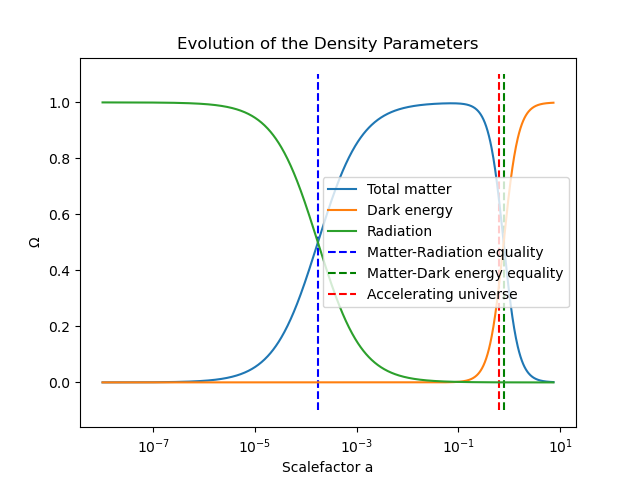
\includegraphics[width=77mm]{Omega.png}
	\caption{Evolution of the density parameters}
	\label{fig:Omega}
\end{figure}
In figure \eqref{fig:Omega} we can see that the evolution of the density parameters. We see that at the beginning the radiation density was the fully dominated density. As the scalefactor increases, the matter density increases as well and gets fully dominant for a period. As we goes towards our time the universe starts to accelerate and the dark energy density gets equal to the matter density, after the scalefactor increases more we see that the dark energy density dominates the universe right now. \\
\begin{figure}[H]
	\centering
	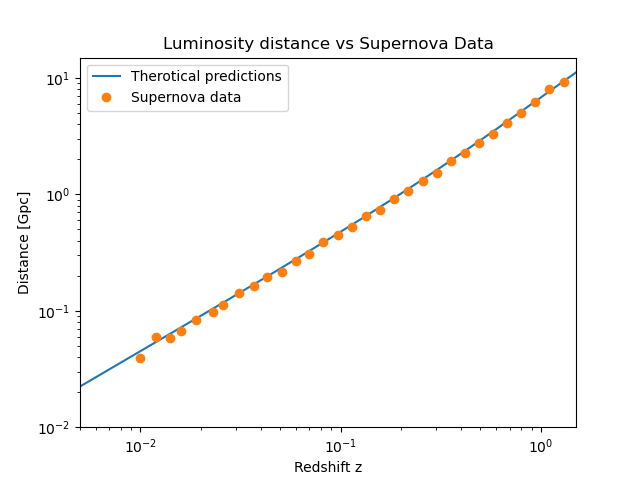
\includegraphics[width=77mm]{LD_vs_SN.png}
	\caption{Theoretical predictions of the luminosity distance compared with supernova data.}
	\label{fig:LD_vs_SN}
\end{figure}
We see that our theoretical predictions fits well with the data we received from the supernova, which makes sense since the errors we got where small.
\end{multicols}
\clearpage
\appendix % Her kommer appendix.

\section{Appendix A}
\label{A.1}
\subsection{$\frac{d\mathcal{H}(x)}{dx}/H$ and $\frac{d^2\mathcal{H}(x)}{dx^2}/H$}
\begin{align*}
    {\mathcal{H}}&=e^xH\\
    &=e^xH_0\sqrt{\frac{\rho_x}{\rho_c}}\\
    &=H_0\frac{1}{\sqrt{\rho_c}}e^{-\frac{3}{2}(1+\omega)+x}\\
    &=\frac{H_0}{\sqrt{\rho_c}}e^{-\frac{1}{2}x-\frac{3}{2}(x\omega}\\
    &=H_0\frac{1}{\sqrt{\rho_c}}e^{-\frac{1}{2}x(1+\omega)}\\
\end{align*}
We now use the $\mathcal{H}$ we got to find $\frac{d\mathcal{H}}{dx}$ 
\begin{align*}
    \frac{d\mathcal{H}}{dx}&=\frac{H_0}{\rho_c}\bigg(-\frac{1}{2}(1+3\omega)\bigg)e^{-\frac{1}{2}x}
\end{align*}
Which finally gives us 
\begin{align}
    {\frac{d\mathcal{H}(x)}{dx}/H}&=\frac{\frac{H_0}{\rho_c}\bigg(-\frac{1}{2}(1+3\omega)\bigg)e^{-\frac{1}{2}x}}{\frac{H_0}{\rho_c}e^{-\frac{1}{2}x}}\\
    &=-\frac{1}{2}(1+3\omega)
\end{align}
We will now find $\frac{d^2\mathcal{H}(x)}{dx^2}/H$, and we do this by first finding the derivative of $\frac{d\mathcal{H}(x)}{dx}$
\begin{align}
    \frac{d^2\mathcal{H}(x)}{dx^2}/H=\frac{H_0}{\sqrt{\rho_c}}\frac{1}{4}(1+3\omega)^2e^{-\frac{1}{2}x} 
\end{align}
Which now gives us $\frac{d^2\mathcal{H}(x)}{dx^2}/H$
\begin{align}
    \frac{d^2\mathcal{H}(x)}{dx^2}/H&=\frac{\frac{H_0}{\sqrt{\rho_c}}\frac{1}{4}(1+3\omega)^2e^{-\frac{1}{2}x} }{\frac{H_0}{\rho_c}e^{-\frac{1}{2}x}}\\
    &=\frac{1}{4}(1+\omega)^2
\end{align}
\clearpage
Link for the code: \url{https://github.com/andreaswetzel/AST5220---Cosmology-II.git}\\
\\
\\
\\
\\
Run code as usual.\\
make clean; make\\
.(backslash)cmb\\
python3 Plot.py         To see the plots\\
\\
NB! Use the 
\bibliography{References} % Kilder.
\begin{thebibliography}{9}
    \bibitem{Dodelson}
    Dodelson Scott - Modern Cosmology 
	\bibitem{Oppgaven}
	Short description, theoretical background - \url{https://cmb.wintherscoming.no/milestone1.php} 
	\bibitem{BC}
	Background cosmology - \url{https://cmb.wintherscoming.no/theory_background.php} 
	\bibitem{Claudia}
    Cicone Claudia - AST2210 Lecture Notes 2 - Radiative processes and Photometry 
\end{thebibliography}
\end{document}
